\documentclass[11pt,letterpaper]{article}
%% Coverpage Packs
\usepackage{wallpaper}

%%Query packs
\usepackage[utf8]{inputenc}
\usepackage{amsmath}
\usepackage{amsfonts}
\usepackage{amssymb}
\usepackage{url}
\usepackage{xcolor}
\usepackage{fullpage}
\usepackage{listings}
\usepackage{mathtools}
\usepackage{enumitem}
\usepackage{bm}
\usepackage{fixltx2e}
\usepackage{hyperref}
\usepackage{array}
\usepackage{multirow}
\usepackage{longtable}

\lstset{
	basicstyle=\ttfamily,
	columns=fullflexible,
	breaklines=true,
	postbreak=\mbox{\textcolor{red}{$\hookrightarrow$}\space},
}
\setlength\parindent{24pt}

%%Graphics packs
\usepackage{ulem}
\usepackage{geometry, tikz}
  \usepackage{graphicx}
\usetikzlibrary{shapes,shadows,arrows.meta}
\geometry{
    a4paper,
    total={170mm,257mm},
    left=20mm,right=20mm,
    top=20mm,
}

%%Assumption/Constraint Packs
\usepackage{enumitem}

\title{Comp353 Project Report}
\author{Kai Nicoll-Griffith[40012407], Stephen Prizio[40001739], \\Giovanni Gebran[40018637], Nizar Belhassan[27519443]\\\\\bf{Team kzc353\_4}}

\begin{document}
	
	

	\begin{titlepage}
\tikz[remember picture,overlay] \node[opacity=1.0,inner sep=0pt] at (current page.center){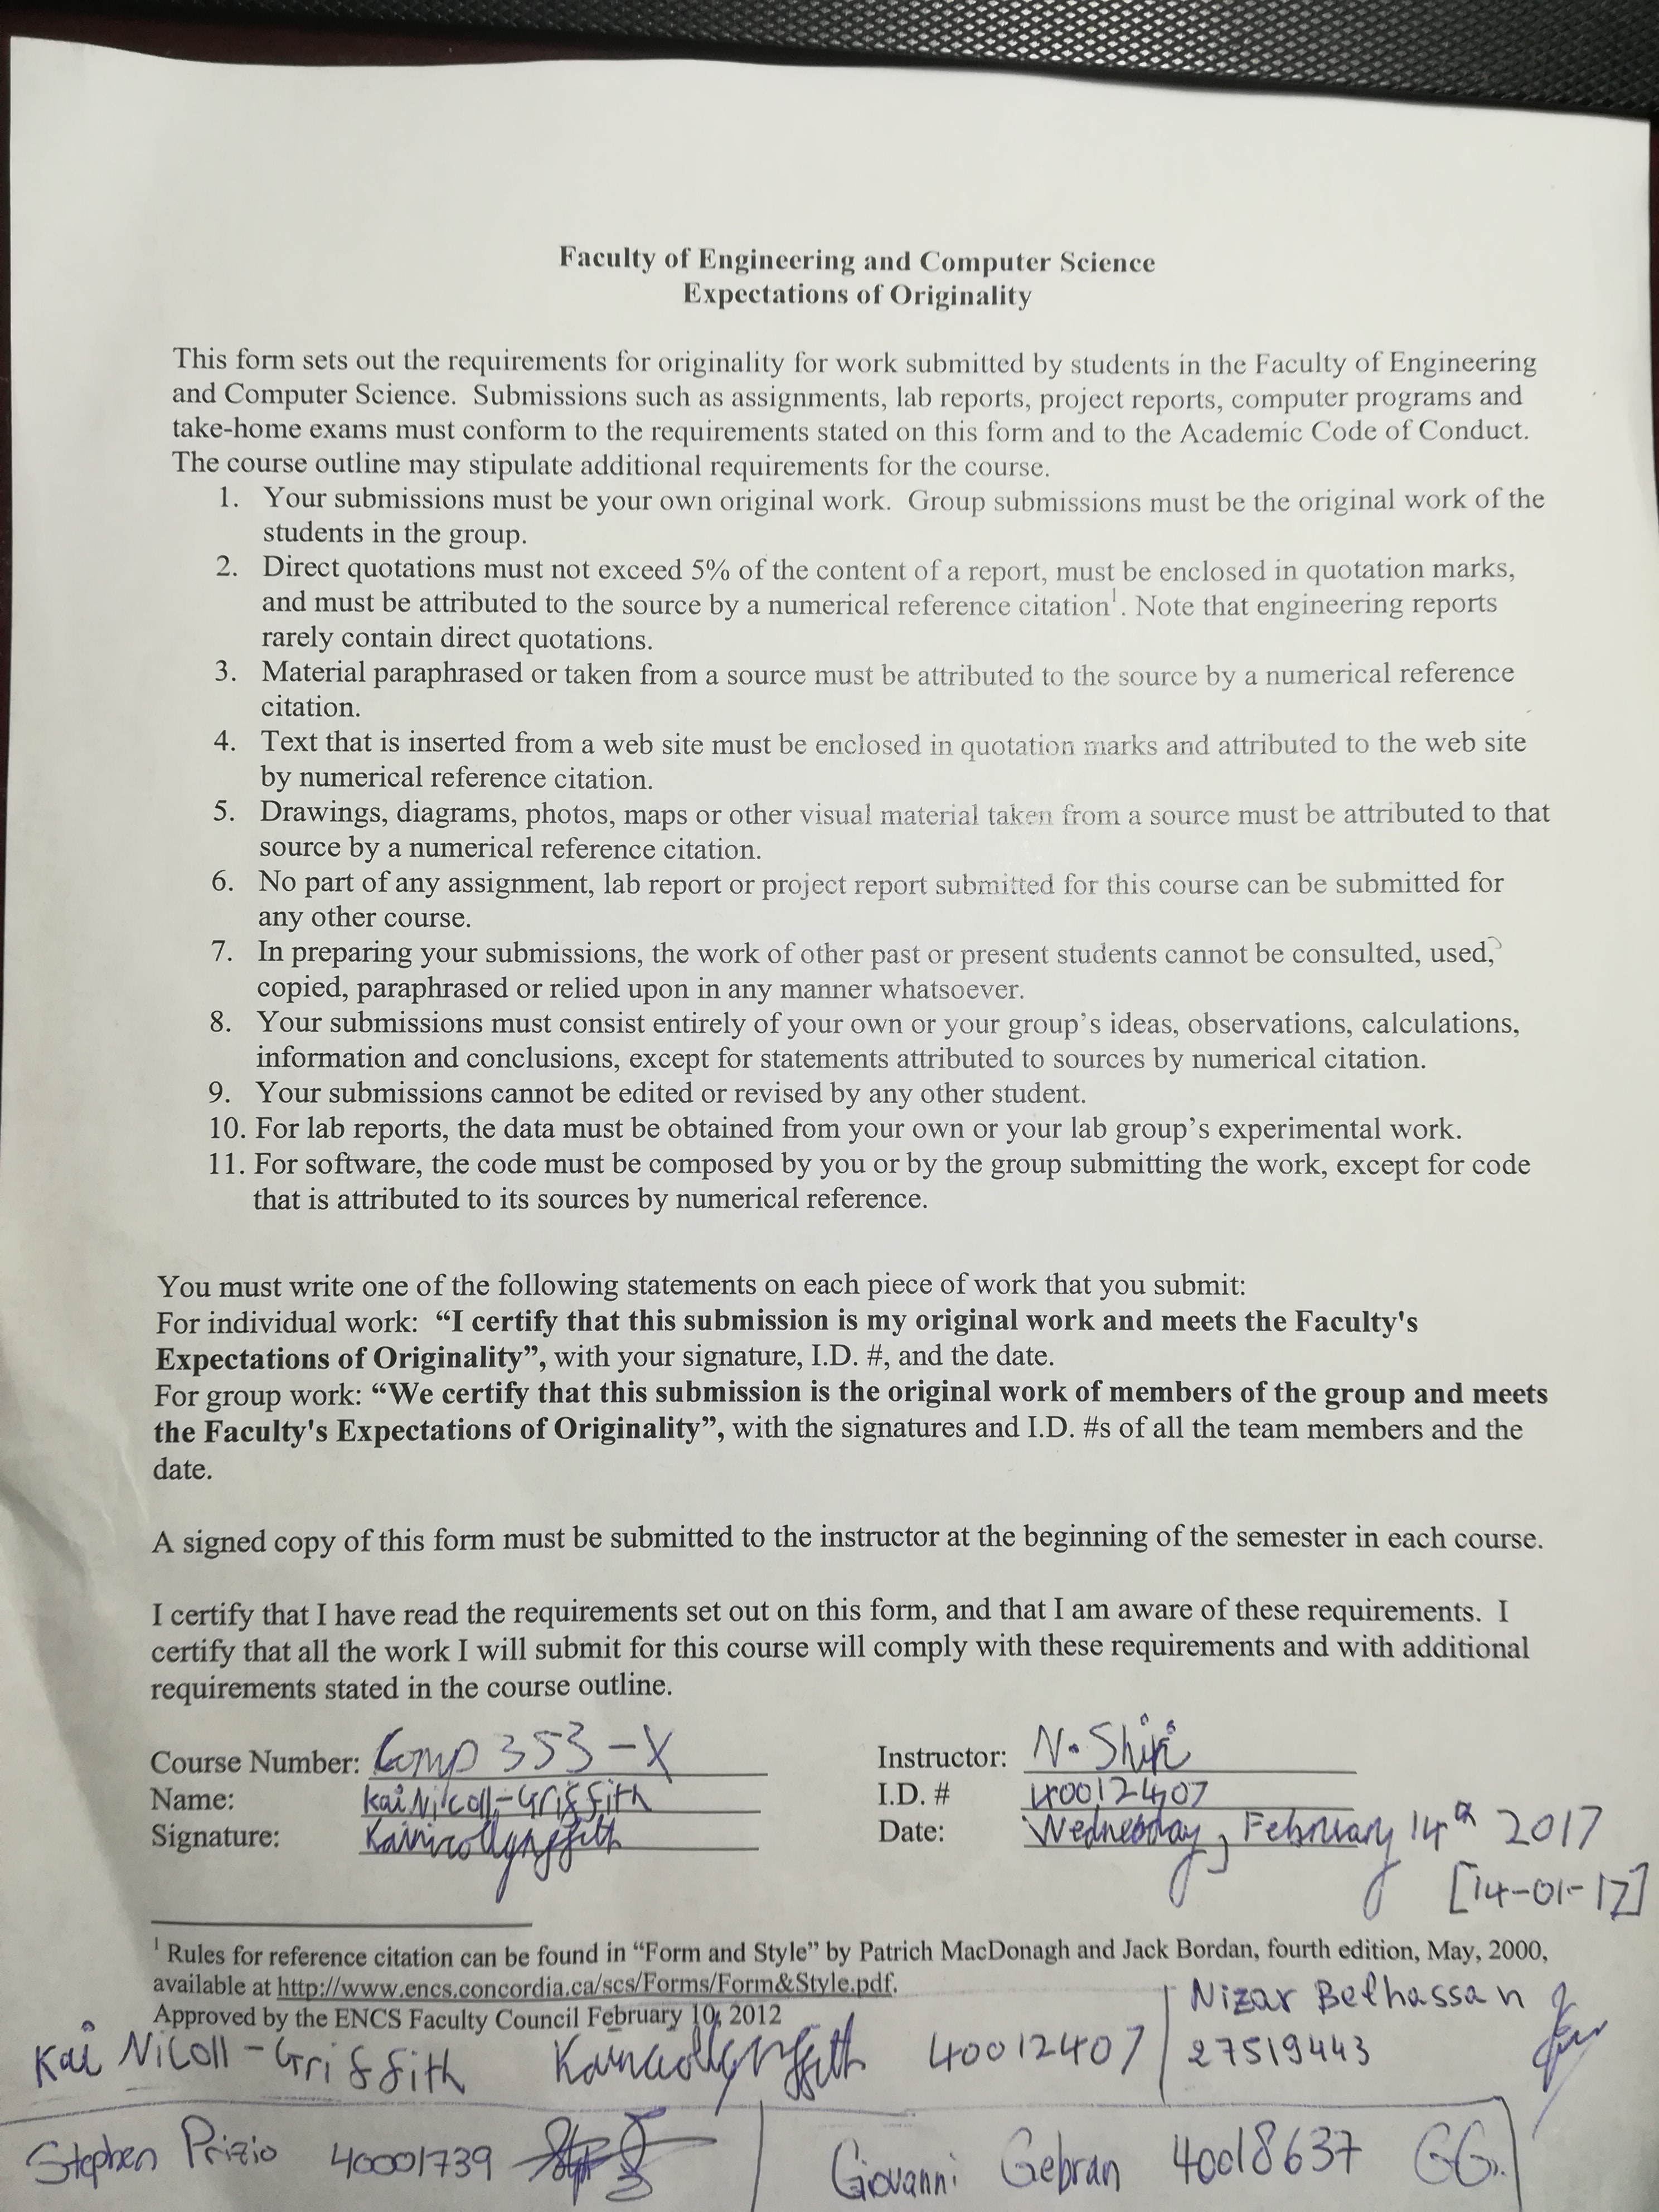
\includegraphics[width=\paperwidth,height=\paperheight]{originality.jpg}};
\end{titlepage}
	
		\maketitle
		\newcommand{\graphicwidth}{18.5cm}
	\section{Entity Relationship Diagram}
\hspace*{-1.1cm}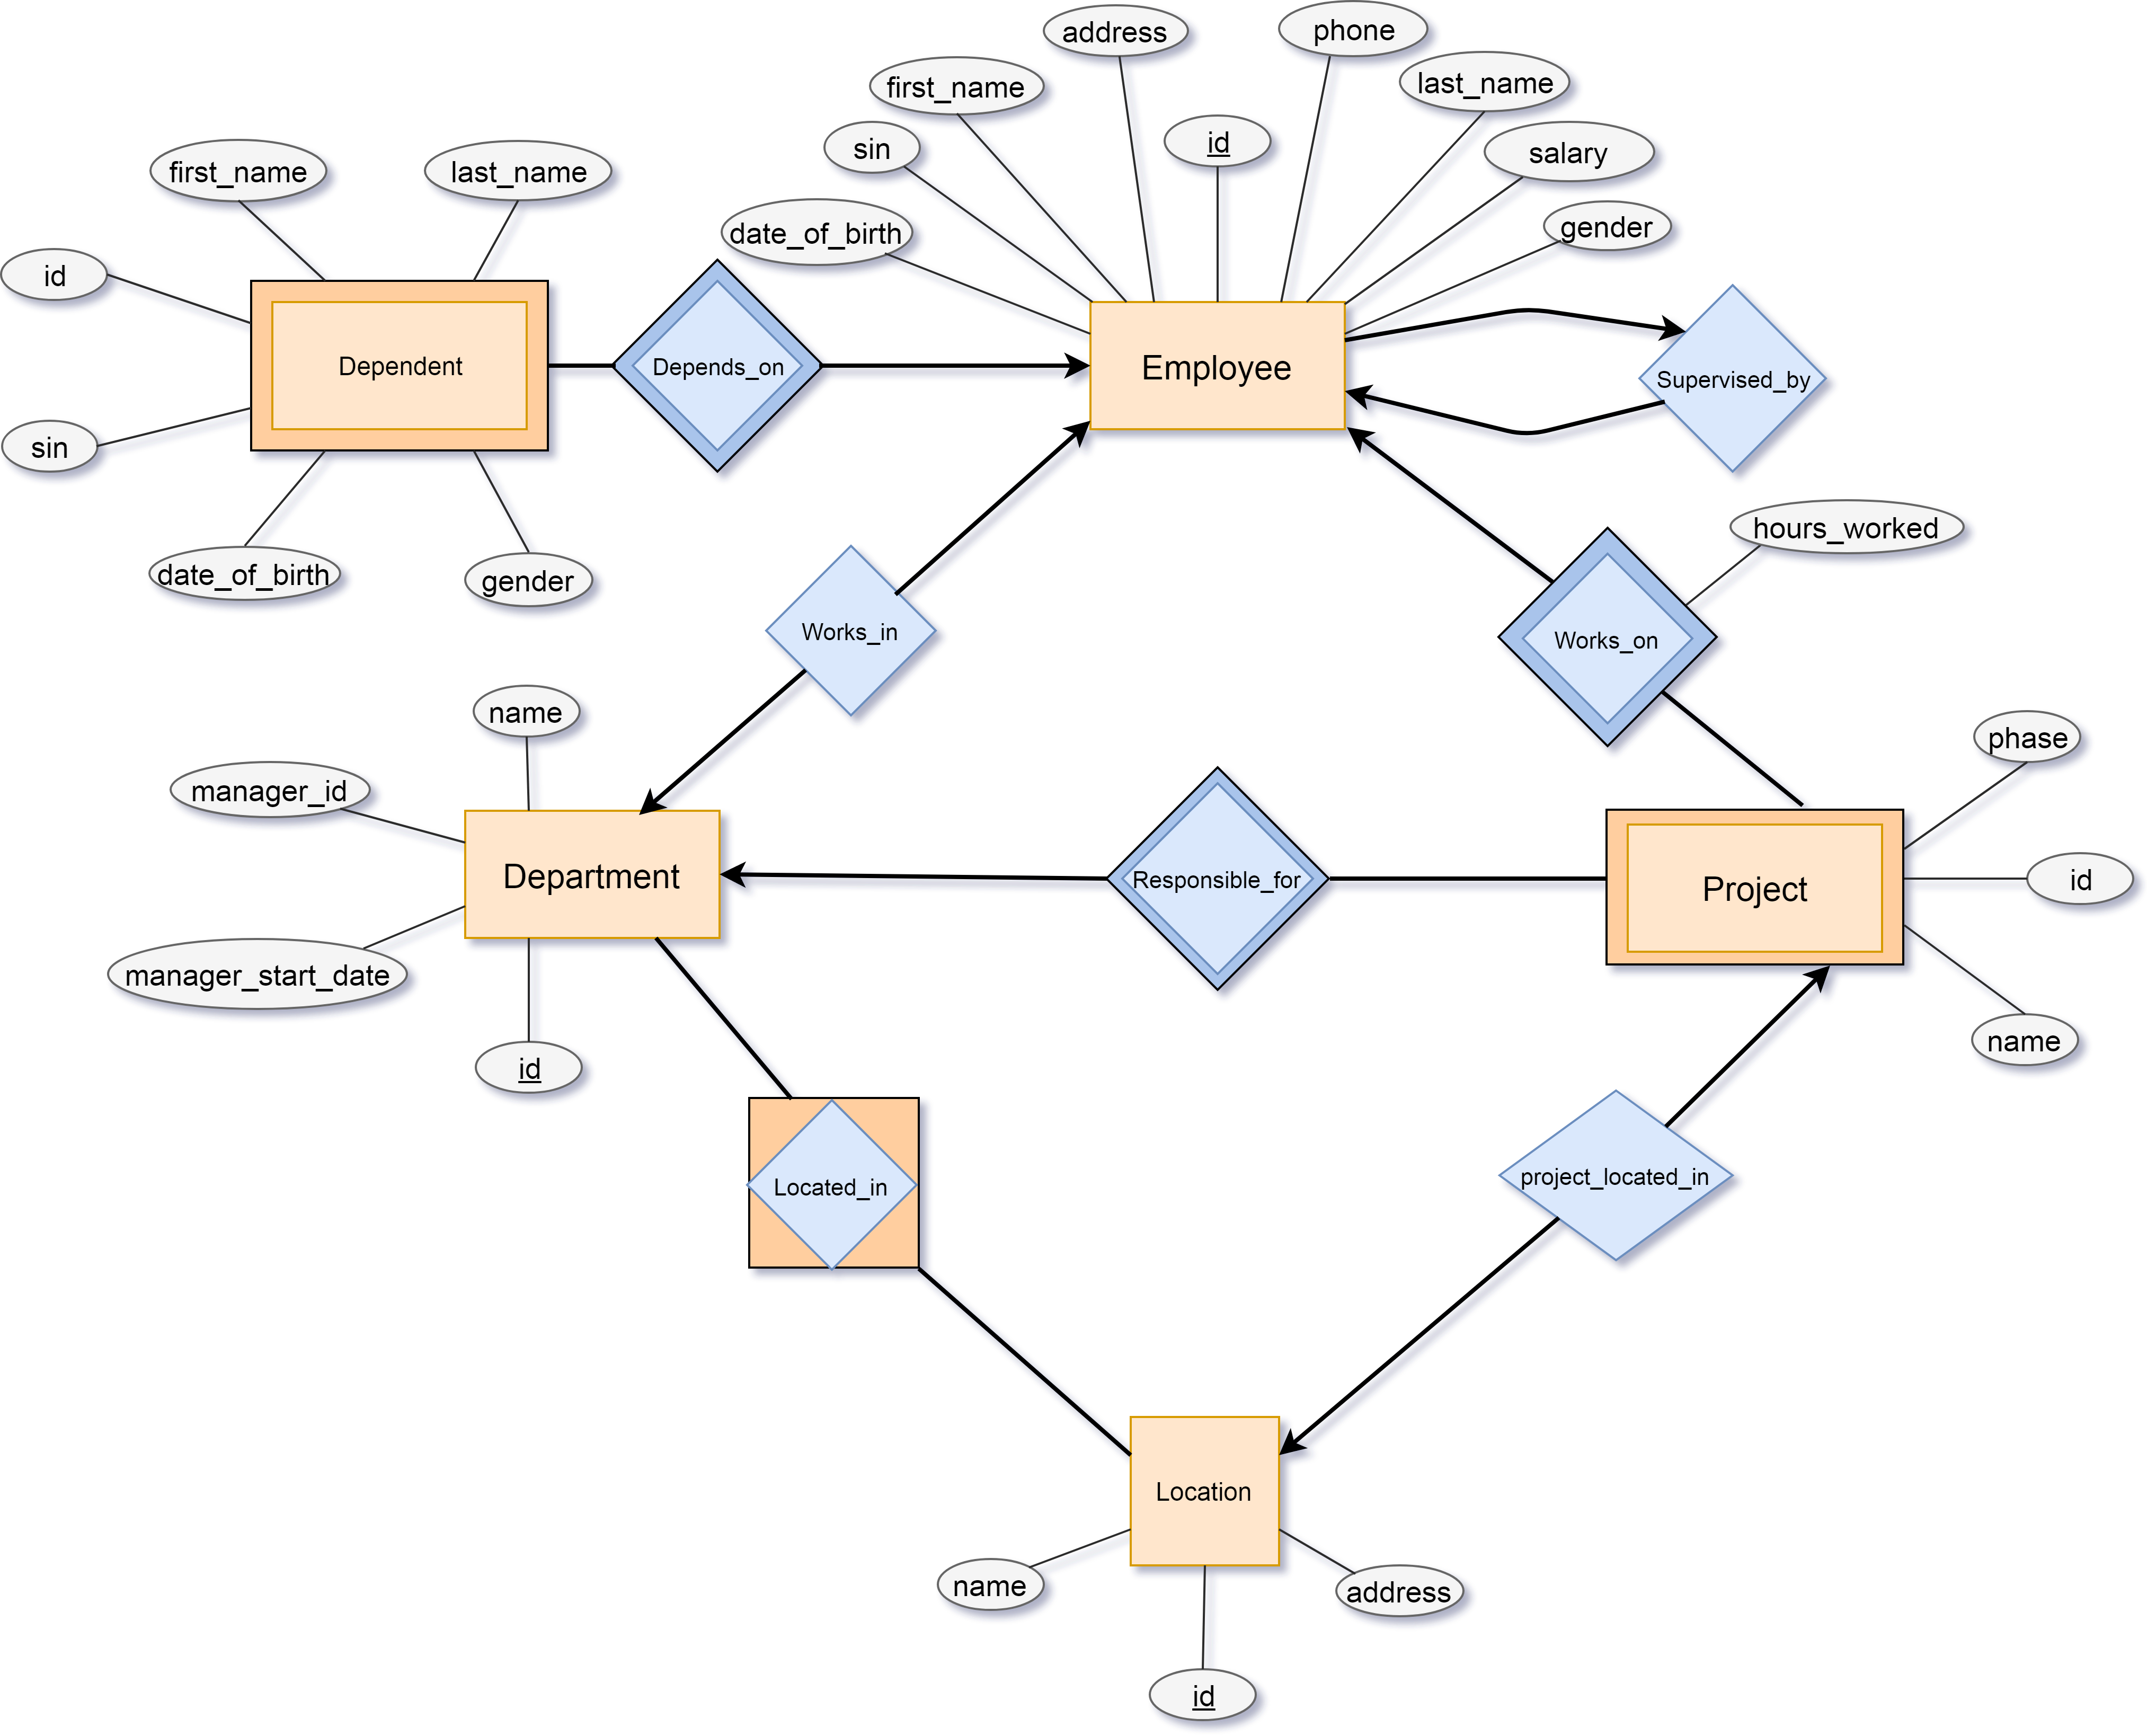
\includegraphics[width=\graphicwidth]{erd.png}
	\section{Reasonable Assumptions}
		\subsection{general cases}
	An assumption is made that all identification numbers are unsigned integers. An \uline{identification key} will never have a sign so the database restricts this. \\	
	
	\subsection{department table}
	In the case of the `department` table, both the \uline{manager\_id} and \uline{manager\_start\_date} are given the opportunity to be null since it is not always true that a `department` needs a manager. Small groups could potentially self manage if that is the policy of the company. \\
	\subsection{employee table}
	To ensure there will always be relevant `employee` data, there are no optional or null possible parameters possible within the `employee`  table. It is assumed that a company needs to keep accurate track of everyone within it and null values would encourage poor data management practice of the company. A \uline{salary}(a 5,2 decimal datatype) is given to each employee in dollars per hour to make certain queries easier to process. Due to legislation, \uline{gender} attribute is defined by one ambiguous character. An `employee` must work for a single `department`.\\
	
		\subsection{project table}
	 It is assumed that a `project` can not be assigned to multiple `departments`. Also a `project` has a varchar \uline{phase} attribute which keeps track of the progress of each individual project within the COMPANY database.\\

		\subsection{dependent table}
The `dependent` table holds vital information that has potential legal importance so none of these fields may be null. A dependent is linked to an `employee` by a foreign key holding \uline{employee\_id} and has the multiplicity of one to many. An `employee` may have many `dependents`. \\

\subsection{location table}
In order to specify where a `project` or `department` is situated, a `location` table keeps track of all of the possible locations where departments and projects operate. An entity table will therefore use a relation table holding an unsigned \uline{location\_id} to specify where the department or project is located in both address and an optional name. The \uline{name} is assumed to be used for employee convenience to identify a location while a mandatory \uline{address} is used for more direct positioning and referencing(as would be used by a post office). The \uline{name} is a varchar, while the \uline{address} is medium text since it is assumed that the address could be as specific as country down to room number and limitations on varchar size could be problematic.\\

\subsection{supervised\_by table}
The `supervised\_by table` defines a role of being a subordinate to someone and helps to give information about the status of an employee in the business hierarchy. Supervision does not imply that an employee is a manager and it could be that an employee both supervises and manages a `department`. It is assumed that this relation is solely used to show the hierarchy of employees within the company. To recognize the `employee` who is supervised, each employee is given a single \uline{supervisor\_id} with a 1:1 multiplicity. Our assumption is that an employee should only be supervised by one person or none at all therefore \uline{employee \_id} is a primary key enforcing uniqueness while \uline{supervisor\_id} is a default null value, where null implies an `employee` is unsupervised.\\

\subsection{depends\_on relation}
	The weak relation  `depends\_on` creates the assumption an `employee` can have many `dependants` in a 1:many relationship.
	
\subsection{works\_on relation}
	The weak relation `works\_on` creates the assumption that an `employee` can work on many `projects` in a 1:many relationship
\subsection{works\_in relation}
The strong relation `works\_in` creates the assumption that an `employee` can only work in one `department` in a 1:1 relationship.
\subsection{responsible\_for relation}
	The weak relation `responsible\_for` creates the assumption that a `department` can be responsible for many `projects` in a 1:many relationship
\subsection{project\_located\_in relation}
The strong relation `project\_located\_in` creates the assumption that a project has to be tied to one location in a 1:1 relationship.
\subsection{department\_located\_in relation}
The associative entity `project\_located\_in` creates the assumption that a `department` can be positioned in many `locations` while at the same time a `location` can be assigned to many `departments` in a many:many relationship.

\section{ER to Relation conversion }

Department(\uline{id}, name, manager\_id, manager\_start\_date)\\
Dependent(\uline{id}, first\_name, last\_name, sin, date\_of\_birth, gender, employee\_id)\\
Employee(\uline{id}, first\_name, last\_name, sin, date\_of\_birth, address, phone, salary, gender, department\_id)\\
Project(\uline{id}, name, location\_id, phase)\\
Location(\uline{id}, name, address)\\
Role(\uline{employee\_id}, \uline{supervisor\_id})\\
Works\_on(project\_id, employee\_id, hours\_worked)\\
Located\_in(location\_id, department\_id)\\
Responsible\_for(department\_id, project\_id)\\
\section {Normalization steps and assumptions}

\section{Implemented Functionalities}
\subsection{Database design}
In the COMPANY database There are three primary categories of entity from which more complex entities are defined. These are:
\begin{enumerate}[]
	\item departments, 
	\item employees,
	\item projects,
\end{enumerate}
Each of these tables specifies information that defines the three main entities in the database. These three main entity sets are also enhanced by the entity sets of:
\begin{enumerate}[]
	\item dependent 
	\item location	
\end{enumerate}	
And also the role relation:
\begin{enumerate}[]	
	\item supervised\_by 	
\end{enumerate}
Which specifies an employees role against other employees as a supervisor.\\
While the entity-relation diagram specifies multiple that multiple possible relations can be made, in order to reduce the complexity of the design(and therefore the queries) only the following relations are used
\begin{enumerate}[]
	\item works\_on
	\item responsible\_for
	\item located\_in
\end{enumerate}
These three relations were deemed most important and the other relations seen on the E/R diagram have been omitted.

\subsection{Language and tools}
	The application makes use of the PHP 5.5.9 language due to it's reliable and simple functions for connecting with a MySQL database. In order to more easily input queries on the database and build a modern looking front end system, Lavarel has been used to make development easier which adds additional functionality to and shortcuts to front-end design.\\

\subsection{Query Functionalities}
	21 Queries allow the system to select, update and add to the company database. These are in the form of .php filenames found in the source code folder.
	\subsubsection{delete\_department.php}
	DELETE FROM department WHERE department.id ='\$id'
	\subsubsection{get\_all\_projects\_for\_department.php}
	SELECT responsible\_for.project\_id AS Project\_ID, (SELECT project.name FROM project WHERE responsible\_for.project\_id=project.id) AS Project\_Name FROM responsible\_for WHERE department\_id = \$department\_id
	\subsubsection{get\_employee\_dependents.php}
	SELECT dependent.id AS Dependent\_ID, dependent.first\_name, dependent.last\_name FROM dependent, employee WHERE dependent.employee\_id='\$employee\_id' AND employee.id=dependent.employee\_id
	\subsubsection{get\_employee\_involved\_in\_least\_num\_of\_projects.php}
	SELECT works\_on.employee\_id, employee.first\_name, employee.last\_name
	FROM works\_on
	JOIN employee
	on employee.id=works\_on.employee\_id
	Group by employee\_id
	Order by COUNT(project\_id) ASC
	LIMIT 1
	\subsubsection{get\_employee\_involved\_in\_most\_num\_of\_projects.php}
	SELECT works\_on.employee\_id, employee.first\_name, employee.last\_name
	FROM works\_on
	JOIN employee
	on employee.id=works\_on.employee\_id
	Group by employee\_id
	Order by COUNT(project\_id) Desc
	LIMIT 1
	\subsubsection{get\_employee\_supervisor.php}
	SELECT role.supervisor\_id AS Supervisor\_ID, (SELECT first\_name FROM employee WHERE role.supervisor\_id=employee.id ) AS First\_Name, (SELECT last\_name FROM employee WHERE role.supervisor\_id=employee.id ) AS Last\_Name FROM role, employee WHERE role.employee\_id='\$employee\_id' AND employee.id=role.employee\_id
	\subsubsection{get\_employees\_who\_work\_on\_a\_project.php}
	SELECT employee.id AS Manager\_ID,employee.first\_name, employee.last\_name FROM department JOIN responsible\_for ON department.id=responsible\_for.department\_id JOIN employee ON employee.id=department.manager\_id JOIN works\_on ON works\_on.project\_id=responsible\_for.project\_id AND works\_on.employee\_id=department.manager\_id
	\subsubsection{get\_hours\_worked\_employee.php}
	SELECT hours\_worked FROM works\_on, employee WHERE employee.id = '\$employee\_id' AND project\_id = '\$project\_id' AND employee.id=works\_on.employee\_id
	\subsubsection{get\_how\_much\_employee\_gets.php}
	SELECT employee.salary FROM employee WHERE employee.id=\$employee\_id
	\subsubsection{get\_project\_location.php}
	SELECT project.location\_id AS Location\_ID, (SELECT location.name FROM location WHERE project.location\_id=location.id) AS Location\_name, (SELECT location.address FROM location WHERE project.location\_id=location.id) AS Address FROM project WHERE project.id =\$project\_id
	\subsubsection{get\_total\_hours\_worked\_for\_project.php}
	SELECT SUM(works\_on.hours\_worked) AS total\_hours FROM works\_on WHERE works\_on.project\_id =\$project\_id
	\subsubsection{get\_total\_pay\_for\_each\_project.php}
	SELECT works\_on.hours\_worked, works\_on.employee\_id, employee.salary From works\_on, employee Where  works\_on.project\_id=2 AND employee.id=works\_on.employee\_id
	\subsubsection{insert\_department.php}
	INSERT INTO department (id, name, manager\_id, manager\_start\_date) VALUES ('\$id','\$name','\$manager\_id','\$manager\_start\_date')
	\subsubsection{insert\_dependent.php}
	INSERT INTO dependent (id, first\_name, last\_name, sin, date\_of\_birth, gender, employee\_id) VALUES ('\$id', '\$first\_name', '\$last\_name', '\$sin', '\$date\_of\_birth','\$gender', '\$employee\_id')
	\subsubsection{insert\_employee.php}
	INSERT INTO employee (id, first\_name, last\_name, sin, date\_of\_birth, address, phone, salary, gender, department\_id) VALUES ('\$id', '\$first\_name', '\$last\_name', '\$sin', '\$date\_of\_birth', '\$address', '\$phone', '\$salary', '\$gender', '\$department\_id')
	\subsubsection{insert\_located\_in.php}
	INSERT INTO located\_in (location\_id, department\_id) VALUES ('\$location\_id', '\$department\_id')
	\subsubsection{insert\_location.php}
	INSERT INTO location (id, name, address) VALUES ('\$id', '\$name','\$address')
	\subsubsection{insert\_project.php}
	INSERT INTO project (id, name, location\_id, phase) VALUES ('\$id', '\$name','\$location\_id', '\$phase')
	\subsubsection{insert\_responsible\_for.php}
	INSERT INTO responsible\_for (project\_id, department\_id) VALUES ('\$project\_id', '\$department\_id')
	\subsubsection{insert\_role.php}
	INSERT INTO role (employee\_id, supervisor\_id) VALUES ('\$employee\_id', '\$supervisor\_id')
	\subsubsection{insert\_works\_on.php}
	INSERT INTO works\_on (project\_id, employee\_id, hours\_worked) VALUES ('\$project\_id','\$employee\_id', '\$hours\_worked')
	
\section{contributions}
\subsection{Giovanni Gebran}
 \begin{itemize}
\item Database Design
\end{itemize}
\subsection{Nizar Belhassan}
 \begin{itemize}
\item Database Design
\item Majority of Queries
\end{itemize}
\subsection{Kai Nicoll-Griffith}
 \begin{itemize}
\item Database Design
\item Database Attribute Refinements
\item Report setup and latex
\item Report: ER Diagram
\item Report: Constraints and assumptions
\item Report: Functionalities and query entry
\end{itemize}
\subsection{Stephen Prizio}
 \begin{itemize}
	\item Database Design
	\item Front end Lazarel design
	\item SQL sample data and database 
	\item Minority of Queries
	\item Report: Query entry
\end{itemize}
\end{document}
